\section{Design}
This section considers the context in which the problem exists and the design of each system and subsystem necessary to visualize and realize a possible solution to solve the problem.

The nature of the system exists primarily in the software domain.
As such, a suitable design architecture is postulated by the C4 model.
This model breaks down the system architecture into different layers of complexity, from a generic high-level system overview down to low-level software abstractions.\cite{vazquez2020c4}

Low-level abstractions are realized with unified modeling language (UML) diagrams. UML diagrams detail the members and methods belonging to classes, and the relationships between those classes in an object-oriented codebase. \cite{petre2013uml}

\subsection{System context and base requirements }
Figure \ref{fig:system_context} depicts the system context in the problem domain.
Project specifications have identified two parties expected to utilze the system - the truck drivers and the fleet managers.
Identified requirements on the solution dictate that truck drivers will use an android application to log data on the system.
In addition, fleet managers must view the logged data and manipulate their fleets via a web application running in a browser.

\begin{figure}[H]
\centering
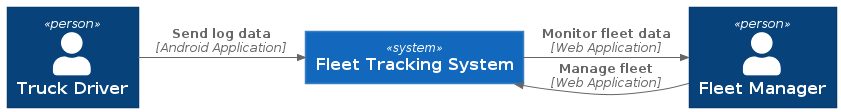
\includegraphics[width=6in]{system_context.png}
\caption{System Context Diagram}
\label{fig:system_context}
\end{figure}

\begin{figure}
\centering
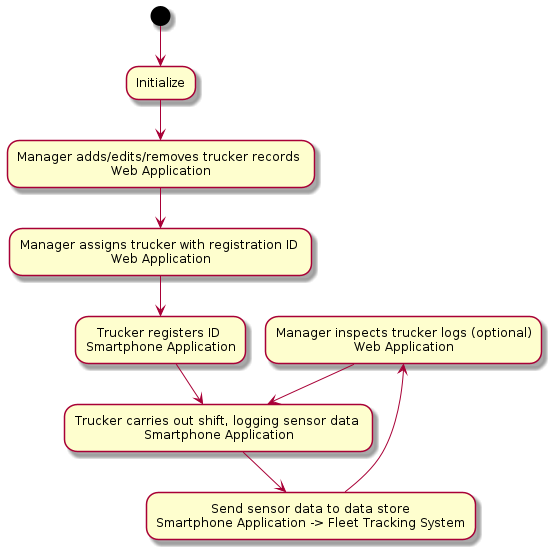
\includegraphics[scale=0.65]{high_level_activity.png}
\caption{System Lifecycle - High Level}
\label{fig:high_level_activity}
\end{figure}
The high-level life cycle view of the fleet-tracking system design is depicted in figure \ref{fig:high_level_activity}.
This life cycle view gives a broad indication of how the system is expected to work for a user.
Only front-end components of the system are considered to clarify exactly how users will interact with the system.

Managers are required to perform initial configuration, as well as adding trucker records to a data store.
After this, truckers may connect to the system and perform their work while allowing their smartphone applications to track the required sensor data. 
This data is then relayed to the system, in which managers may analyze and inspect data logs.

\subsection{Contained subsystems and choice of tools}
The second level of the C4 model identifies the choice of technologies to be utilized to realize the fleet tracking system.
The fleet-tracking system is divided into mostly-independent containers, as depicted in figure \ref{fig:container}.
Each container is a standalone process which makes calls to other processes in the system.
The main choice of software tools are identified for each container.

Truckers will make use of an android data-logging application to fetch the various sensor data, and securely transmit this data via an SSL connection.
The IO server, implemented in C++, will listen for multiple asynchronous connections from the android application and relay the data to a MySQL database.
A web application, realized with the ASP.NET framework fetches the data and allows the fleet manager to view the whereabouts of each member in his/her fleet.
\begin{figure}[H]
\centering
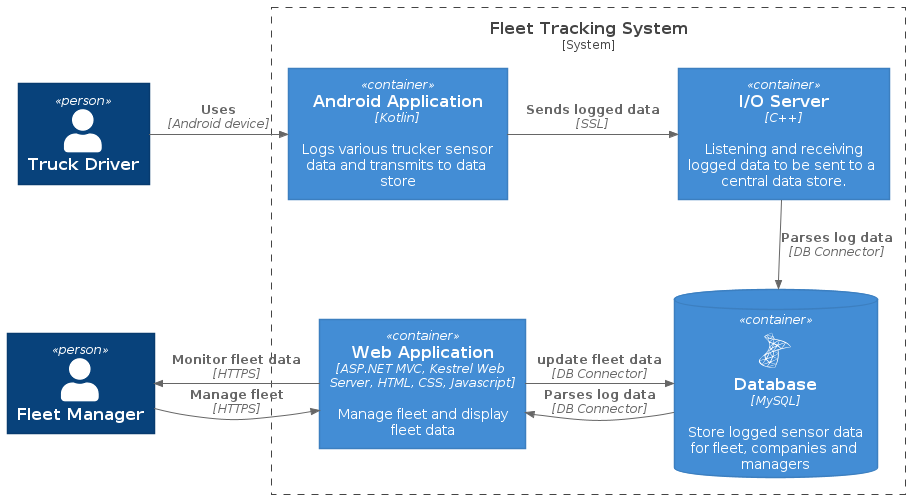
\includegraphics[width=6in]{container.png}
\caption{Container Diagram - Fleet tracking system}
\label{fig:container}
\end{figure}

\subsubsection{Data Model}
The entire system revolves around the effective abstraction and manipulation of logged fleet data.
MySQL is chosen as the RDBMS to realize a relational database model, as it is high performance and reliable.
Other database systems offer comparable performance, but MySQL is chosen for familiarity.

The relational model is depicted in figure \ref{fig:ERD_Overview}.
The model is designed to allow one company to have many managers and truckers. Each trucker can have many logs.

\subsubsection{Android Application}
Kotlin is the language of choice to write the android application due to its simplicity and mainstream Google support.

Truckers must receive an initial code from their managers' to register their devices.
Sensor readings are taken every two minutes, and stored into a lightweight database.
Finally, a connection is attempted with an I/O server. If available, the database contents is emptied into via the I/O server to the central system database.

\subsubsection{I/O Server}
C++ is chosen for the I/O server, due to its high performance capabilities.
The I/O server needs to listen and allow multiple asynchronous connections, during which log data is transmitted to the database.

\subsubsection{Web Application}
The model-view-controller (MVC) architecture will be realized with the Microsoft ASP.NET framework.
This architecture allows for separation between business-logic, data models and viewing logic.
This is necessary to ensure that code related to displaying data is not mixed with code used for core logic, thereby separating and modularizing the functionality of different components in the system.

\subsection{Subsystem components}
Each container in figure \ref{fig:container} is subdivided into several core software components necessary to achieve the desired outcomes.
This is depicted through container diagrams, which makes up the third level of the C4 model.

\subsubsection{Android Application}
The expected life cycle of the Android application is depicted in figure \ref{fig:android_activity}.
Initially, a check is performed to confirm that the trucker ID is in the central database, and is not duplicated.
If this ID is not valid, the trucker must request a valid ID from the fleet manager.

After this, the usual logging process is continued.
Data is polled from the available sensors and stored in a local database.
A connection is attempted with the I/O server and the local database entries are transmitted to the server.
Upon successful transmission, the local database is emptied.

However, if a connection fails, the local database is not cleared.
This process loops continuously loops every two minutes.
 
\begin{figure}[H]
\centering
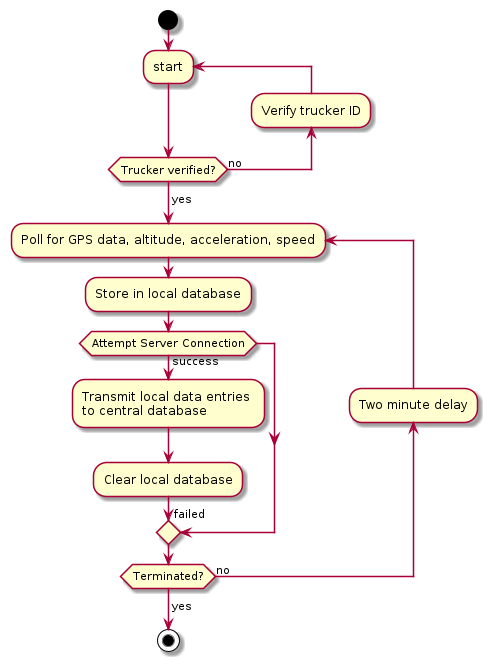
\includegraphics[scale=0.6]{android_activity.png}
\caption{Life-cycle - Android Application}
\label{fig:android_activity}
\end{figure}

Figure \ref{fig:android_component} depicts the system components necessary to realize the required functionality.
The logging controller collects sensor information and interacts with the local database and central I/O server.
Various Android APIs are accessible and expose Location and sensor information to the Logging controller.
\begin{figure}[H]
\centering
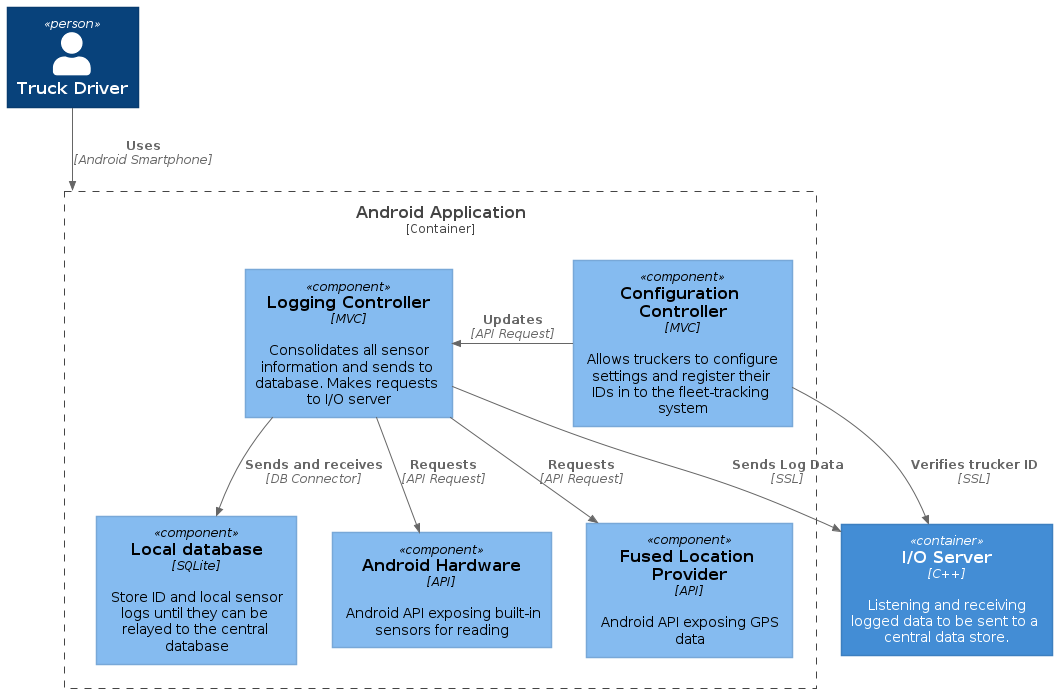
\includegraphics[width=6in]{android_component.png}
\caption{Component Diagram - Android Application}
\label{fig:android_component}
\end{figure}

\pagebreak
\subsubsection{I/O Server}
The typical life cycle view of the I/O server is depicted in figure \ref{fig:IO_activity}.
A secure connection must be made due to the sensitive nature of GPS data.

The I/O server contains a request handler to process the request sent by the android client.
It then calls the specific function as determined and parses the appropriate data via the JSON format.
\begin{figure}[H]
\centering
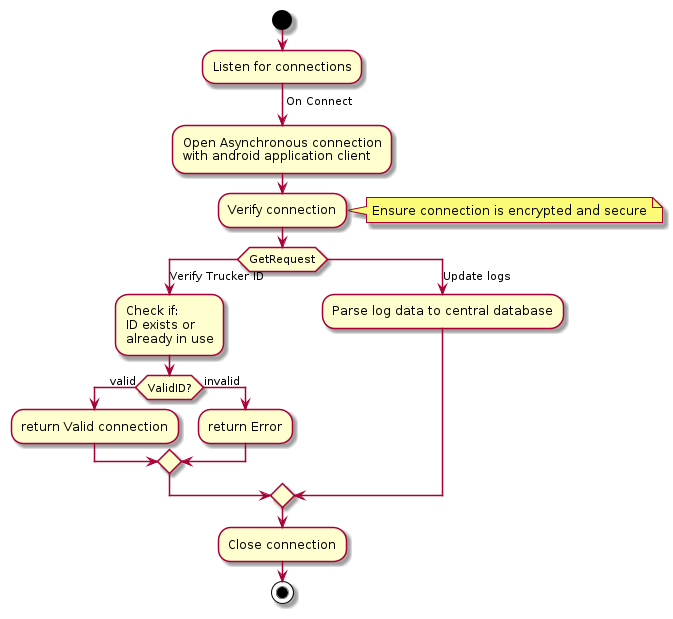
\includegraphics[width=6in]{IO_activity.png}
\caption{Life cycle - I/O Server}
\label{fig:IO_activity}
\end{figure}

\begin{figure}[H]
\centering
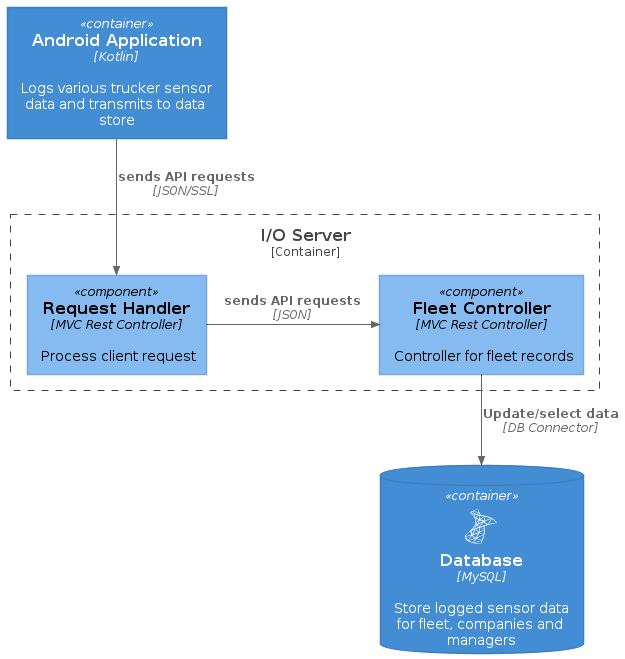
\includegraphics[width=6in]{IO_component.png}
\caption{Component Diagram - I/O Server}
\label{fig:IO_component}
\end{figure}

Figure \ref{fig:IO_component} depicts the component make-up of the I/O server.
The codebase clearly contains these low-level abstractions.

\pagebreak
\subsubsection{MySQL Database}
The MySQL database is driven by MySQL server.
A relational data structure is utilized, as shown in figure \ref{fig:ERD_Overview}.
Relational modelling allows for logical structuring and integrity of the data.
\begin{figure}[H]
\centering
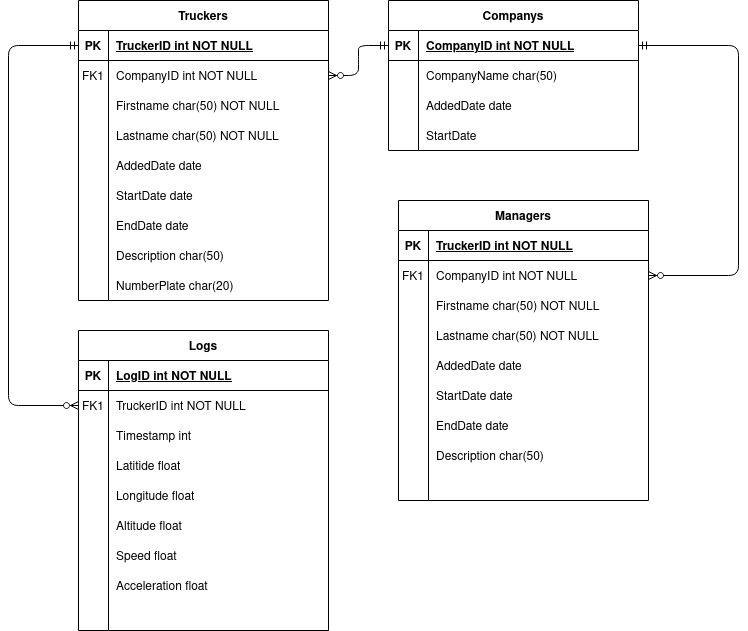
\includegraphics[width=6in]{ERD_Overview.png}
\caption{Entity Relationship Diagram}
\label{fig:ERD_Overview}
\end{figure}

\subsubsection{Web Application}
The web application is modeled with the view-model-controller design pattern, which allows separation of UI logic from business logic.
Two view models are considered to allow for managers to sign in and manage their fleets.
Controllers handle core logic behind the presentation of data.
The central database is also accessed by the controller.
Figure \ref{fig:webapp_component} depicts the architectural arrangement of the web application.

\begin{figure}
\centering
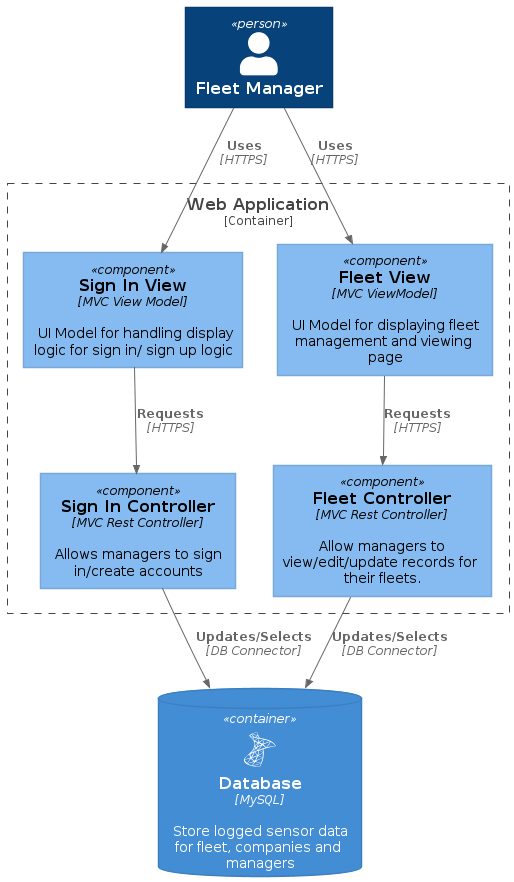
\includegraphics[scale=0.6]{webapp_component.png}
\caption{Component Diagram - Web Application}
\label{fig:webapp_component}
\end{figure}
